
%%%%%%%%%%%%%%%%%%%%%%% file typeinst.tex %%%%%%%%%%%%%%%%%%%%%%%%%
%
% This is the LaTeX source for the TDPTemplate using
% the LaTeX document class 'llncs.cls' Springer LNAI format
% used in the RoboCup Symposium submissions.
% http://www.springer.com/computer/lncs?SGWID=0-164-6-793341-0
%
% It may be used as a template for your own TDP - copy it
% to a new file with a new name and use it as the basis
% for your Team Description Paper
%
% NB: the document class 'llncs' has its own and detailed documentation, see
% ftp://ftp.springer.de/data/pubftp/pub/tex/latex/llncs/latex2e/llncsdoc.pdf
%
%%%%%%%%%%%%%%%%%%%%%%%%%%%%%%%%%%%%%%%%%%%%%%%%%%%%%%%%%%%%%%%%%%%

\documentclass[runningheads,a4paper]{llncs}

% document input
\usepackage[utf8]{inputenc}		% input encoding
\usepackage[english]{babel}		% input language for hyphens

% fonts 
\usepackage[T1]{fontenc}		% more glyphs and a
\usepackage{lmodern}			% better looking font

\usepackage{amssymb}
\setcounter{tocdepth}{3}
\usepackage{graphicx}
\usepackage{amssymb}
\usepackage{url}
\usepackage{float}
\usepackage{amsmath}
\usepackage{graphicx}
\usepackage{wrapfig}
\usepackage{subfigure}
\usepackage{listings}

% *** MORE GRAHPICS ***
\usepackage[usenames,dvipsnames]{color}     

% *** BIBLIOGRAPHY PACKAGES ***
%\usepackage{natbib}     

%%%%%%%%%%%%%%%%%%%%%%%%%%%%%%%%%%%%%%%%%%%%%%%%%%%%%%%%%%%%%%%%%%%
\usepackage{booktabs}           % For tables (toprule, midrule, bottomrule)
\usepackage{todonotes}			% should be defined after the color package
%%%%%%%%%%%%%%%%%%%%%%%%%%%%%%%%%%%%%%%%%%%%%%%%%%%%%%%%%%%%%%%%%%%

%%%%%%%%%%%%%%%%%%%%%%%%%%%%%%%%%%%%%%%%%%%%%%%%%%%%%%%%%%%%%%%%%%%
% *** PATHS ***
\makeatletter
\def\input@path{{Figures/}		
				}
\makeatother

\graphicspath{  {Figures/}
				}
%%%%%%%%%%%%%%%%%%%%%%%%%%%%%%%%%%%%%%%%%%%%%%%%%%%%%%%%%%%%%%%%%%%

%%%%%%%%%%%%%%%%%%%%%%%%%%%%%%%%%%%%%%%%%%%%%%%%%%%%%%%%%%%%%%%%%%%

% Acronym definitions
\usepackage[acronym,nomain,toc]{glossaries}
\newacronym{ed}{ED}{Environment Descriptor}
\newacronym{fcfg}{FCFG}{feature context free grammar}

% shorthand definitions
\newcommand{\eg}{\emph{e.g.}}						% Exemplum gratia
\newcommand{\goal}{\mathcal{G}}						% Goal area
\newcommand{\goallc}{\mathcal{G}_{\mathrm{lc}}}		% Subset of goal area with costs below threshold cmin
\newcommand{\goalhc}{\mathcal{G}_{\mathrm{hc}}}		% Subset of goal area with costs above threshold cmin
\newcommand{\ie}{\emph{i.e.}}						% Id est
%%%%%%%%%%%%%%%%%%%%%%%%%%%%%%%%%%%%%%%%%%%%%%%%%%%%%%%%%%%%%%%%%%%

\begin{document}

\title{Tech United Eindhoven @Home 2016 Team Description Paper}
\author{J.J.M.~Lunenburg, S.~van~den~Dries, R.P.W.~Appeldoorn, R.W.J.~Wijnands and M.J.G.~van~de~Molengraft}
\institute{Eindhoven University of Technology,
\newline Den Dolech 2, P.O. Box 513, 5600 MB Eindhoven, The Netherlands\\
\texttt{http://www.techunited.nl, techunited@tue.nl}}
\authorrunning{J.J.M.~Lunenburg et al.}

%\author{Team Leader \and Team Members }
%\institute{[Intitute name and direction here], \\
%\texttt{http://devoted-web-site.url}}
\maketitle


%%%%%%%%%%%%%%%%%%%%%%%%%%%%%%%%%%%%%%%%%%%%%%%%%%%%%%%%%%%%%%%%%%%%%%%%%%%%%%%%%%%%

\begin{abstract}
%In your abstract, please state which is the main research line of your team for this year (on which problem or set of problems are you focusing all the team efforts). Tell why this research is important, how are you approaching to the problem solution and which results do you expect to obtain.
This paper provides an overview of the main developments of the Tech United Eindhoven RoboCup@Home team. 
Our main research efforts this year have focused on i) fitting furniture objects to update our object-oriented world model, thereby improving localization, navigation and object segmentation ii) developing a WebGUI to provide the user with a platform-independent way to interact with the robot and iii) natural language interpretation to ease the specification of written commands for the robot and to make speech recognition more robust.
\end{abstract}


%%%%%%%%%%%%%%%%%%%%%%%%%%%%%%%%%%%%%%%%%%%%%%%%%%%%%%%%%%%%%%%%%%%%%%%%%%%%%%%%%%%%

\section{Introduction}
Tech United Eindhoven is the RoboCup team of the Eindhoven University of Technology, competing in the Middle Size League and the @Home League. Tech United has been competing in the @Home league since 2011, winning the 2016 RoboCup European Open and finishing runner-up at RoboCup~2016 in Leipzig.
% in last years' competions.
Tech United Eindhoven consists of (former) PhD and MSc students and staff members from different departments within the Eindhoven University of Technology.

This Team Description Paper is part of the qualification package for RoboCup 2017 in Nagoya, Japan and describes the current status of the @Home activities of Tech United Eindhoven.
Our main research efforts this year have focused on improved object detection via deep learning methods.
%Our main research efforts this year have focused on TODO%fitting furniture objects to update our object-oriented world model (Section~\ref{sec:wmfitting}), developing a WebGUI to provide the user a platform-independent way to interact with the robot (Section~\ref{sec:webgui}) and natural language interpretation (Section~\ref{sec:nli}).


\section{World Model Furniture Fitting}\label{sec:wmfitting}
To successfully solve a RoboCup@Home challenge, a robot needs a basic understanding of the environment: it needs to know how to get from A to B without colliding, it must be able to detect humans and objects with which it has to interact and it must localize itself with respect to the objects it has to manipulate. Therefore ED (Environment Descriptor), a 3D, object-based, volumetric world model was developed. The datastructures and algorithms used in this world model are described in the 2015 TDP (TODO: ref). More information and tutorials can be found on our Github page \footnote{\texttt{https://github.com/tue-robotics/ed}}.

ED depends on having an accurate description of the world, including locations of walls and furniture. However, tables, chairs and even cabinets may move in a household environment. If the world model is not updated accordingly, two important problems arise in a RoboCup@Home setting:

\begin{itemize}
    \item The robot will not position itself correctly with respect to the furniture (cabinet, table, etc) when it needs to interact with or inspect these entities
    \item Since ED uses background subtraction for object segmentation, segmentation may not work correctly
\end{itemize}

\begin{figure}[ht]
        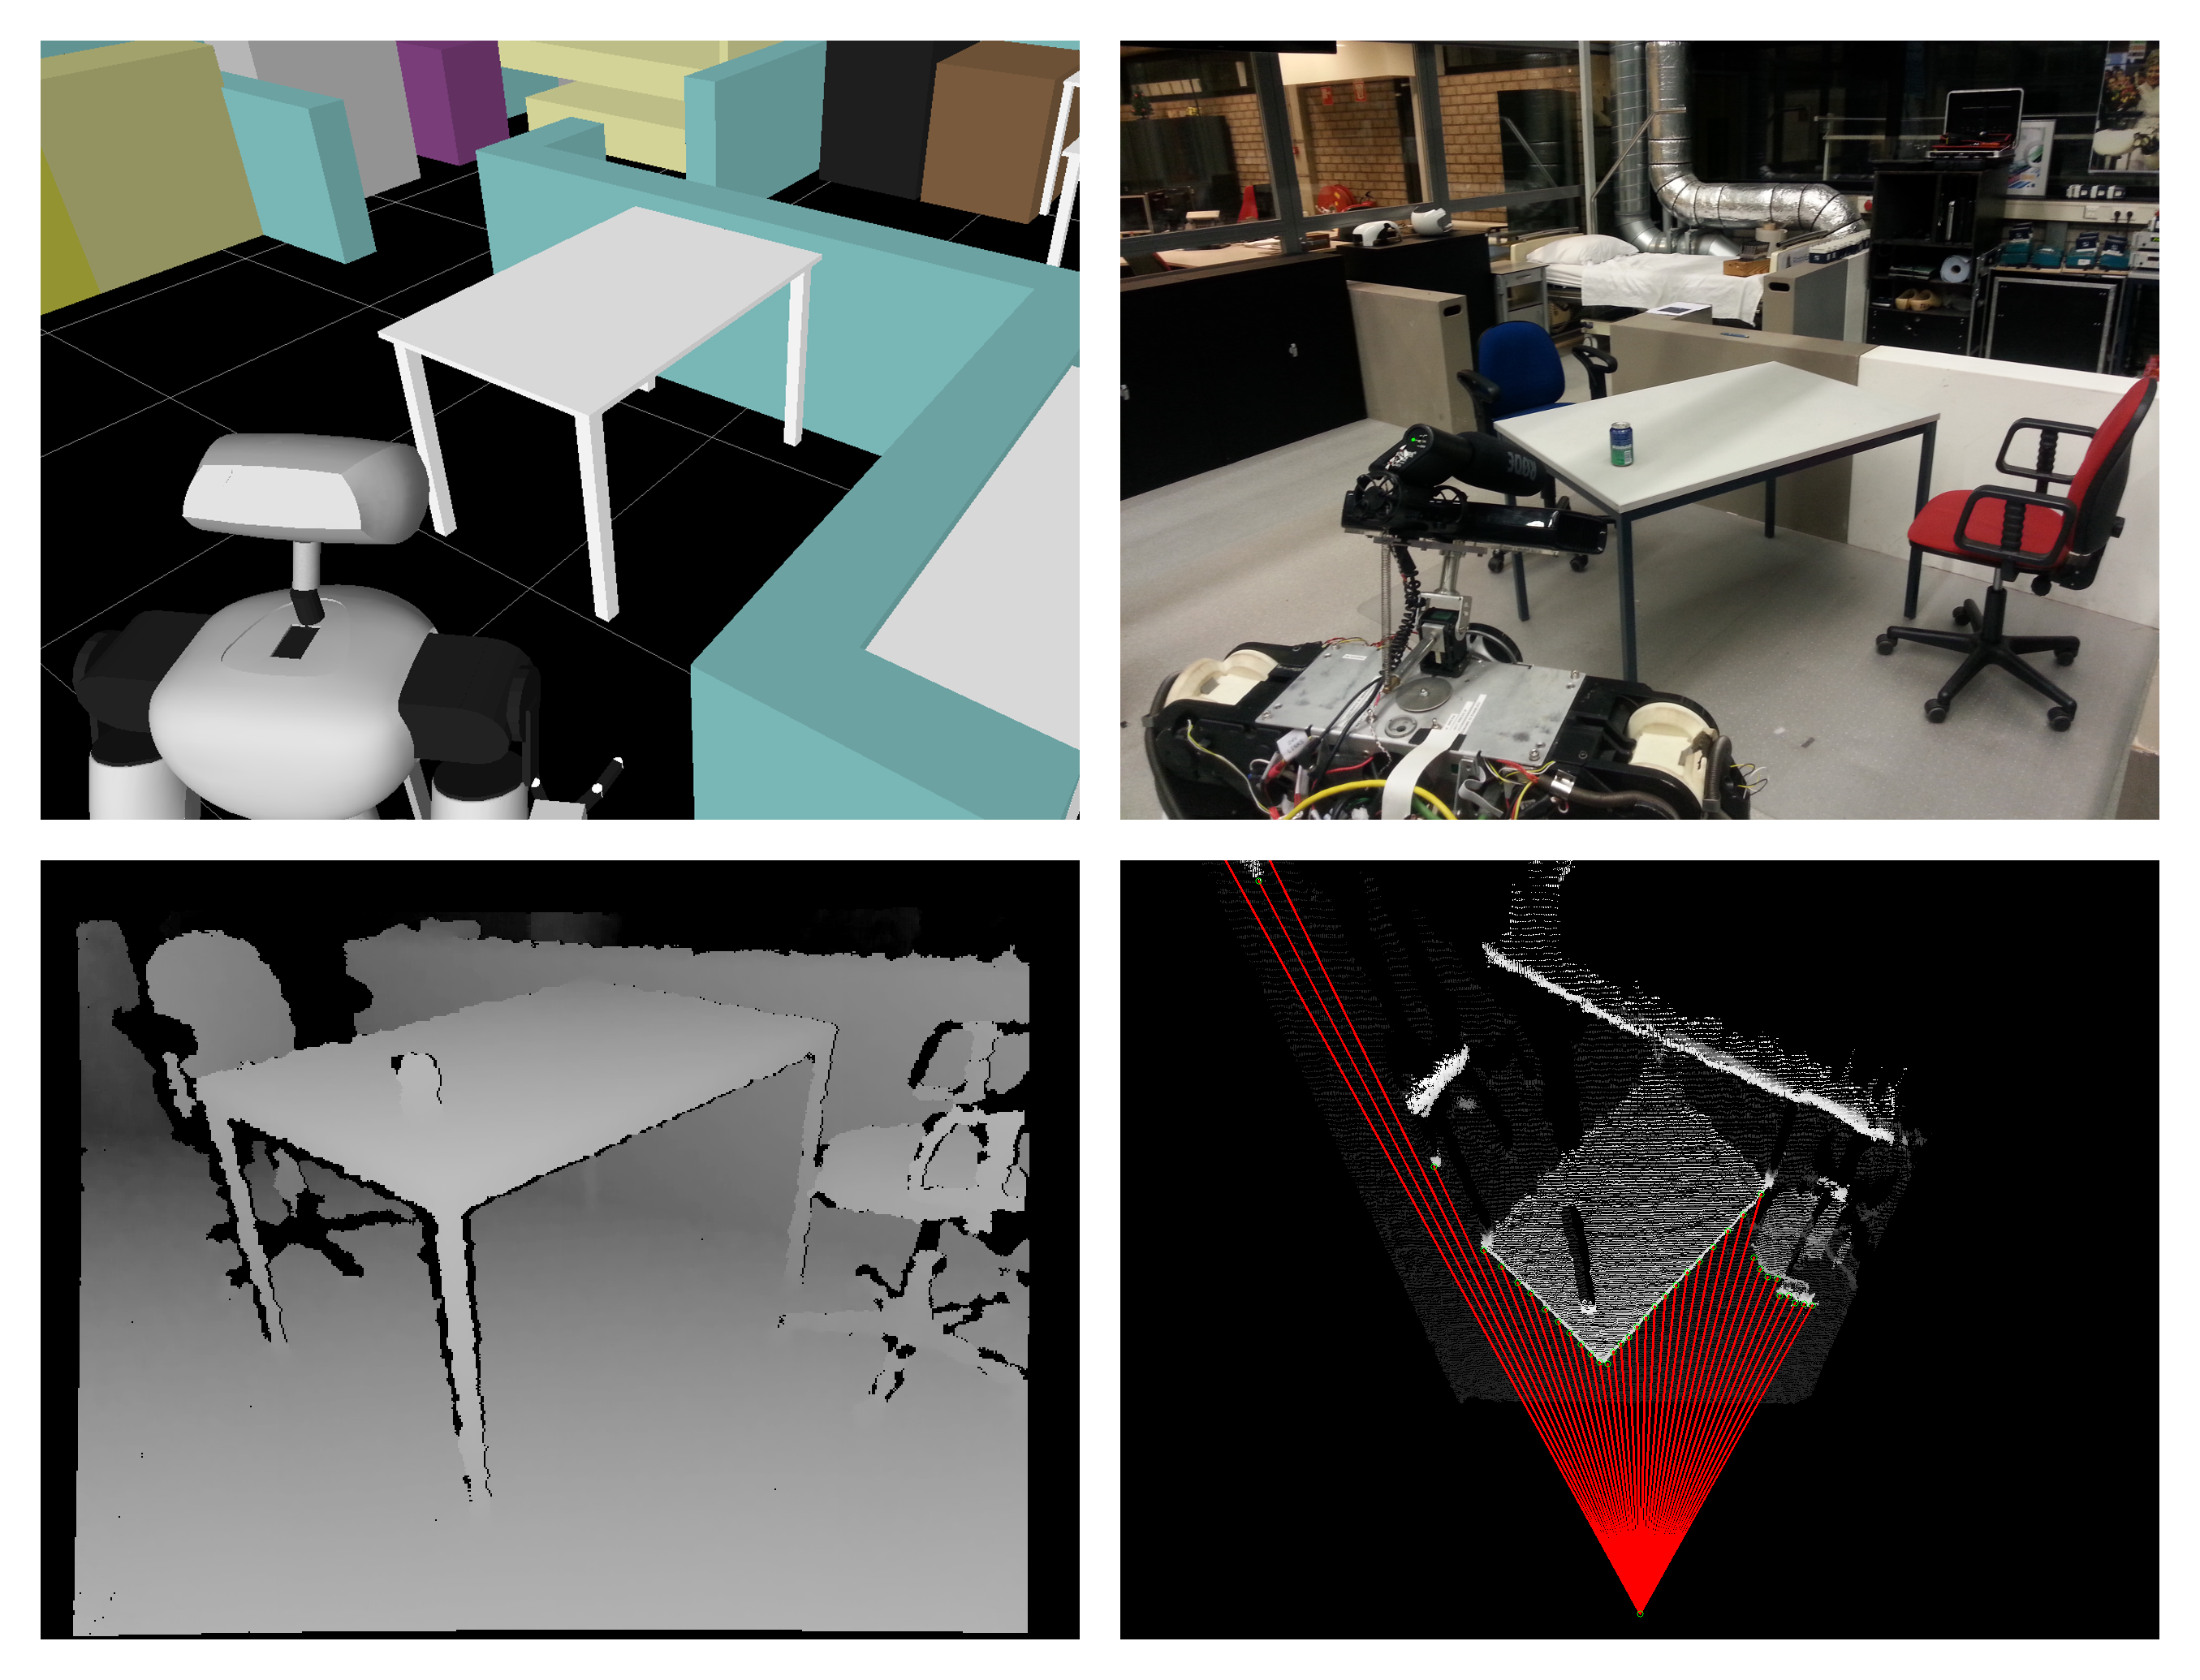
\includegraphics[width = \linewidth]{Figures/fitting}
        \caption{World model furniture fitting algorithm. Top-left: world model visualization as the robot thinks the world is. Top-right: actual situation: the table is rotated and moved. Bottom-left: depth image obtained from the depth sensor (brighter means closer). Bottom-right: top-down projected point cloud (brighter means closer); dividing the points into beams, 2D range data can be extracted and used for efficient template fitting.}
        \label{fig:fitting}
\end{figure}

To deal with this, and to get rid of pre-defined location definitions in general, an ED-plugin was developed which can estimate the positions of furniture in the room. This pose estimation algorithm works as follows (also see Figure~\ref{fig:fitting}):

\begin{enumerate}
    \item The camera pose with respect to the floor is obtained using the robot location and forward kinematics
    \item The point cloud obtained from the depth camera is transformed to the robot's base frame using the camera pose
    \item All points belonging to the floor are filtered using a simple height check per point. All other points are projected onto the floor (resulting in a top-down view).
    \item Then, all projected points are divided into beams that originate at the camera origin. The closest point per beam is stored. This results in a 1-dimensional array of ranges, very similar to the sensor data obtained from a laser range finder. However, the ranges obtained from this algorithm do not simply represent a planar cross-section of the world, but a projection of all points except the ground. This allows the data to also correctly represent a table (while a laser range finder would probably scan above or below the table top)
    \item A top-down 2D contour model is created from the 3D model that needs to be fitted into the sensor data
    \item A simple template-matching algorithm is used to fit the 2D contour model into the 1-dimension range data, resulting in the 2D-pose (x, y, yaw) of the model 
\end{enumerate}

The conversion from a 3D point cloud to a 1-dimension range array enables the use of a very efficient fitting algorithm, which allows for constant tracking of entities at high update rates. Do note, however, that the following assumptions are made:

\begin{itemize}
    \item The entity that needs to be fitted is standing on the ground, and is merely translated along the floor plane, and rotated along the vertical axis (only yaw, no roll or pitch)
    \item The entity is not occluded for large parts by other entities
    \item A 2D top-down contour model is available, or can be constructed from a 3D model
\end{itemize}

Fortunately, these assumptions hold in many situations when trying to estimate the poses of furniture. Several experiments in real situations have shown that the fitting strategy is indeed efficient and effective in many situations.

\section{WebGUI}\label{sec:webgui}
\subsection*{Overview}

In order to interact with the robot aside of speech, a web-based Graphical User Interface (GUI) has been designed. An HTML5 website \footnote{\texttt{https://github.com/tue-robotics/tue\_mobile\_ui}} is hosted on the robotic platform that offers a GUI to multiple users on different platforms with use of a Robot API\footnote{\texttt{https://github.com/tue-robotics/robot-api}} implemented in Javascript. Figure \ref{fig:webgui_architecture} shows an overview of how the user can interact with the robot via this interface.

\begin{figure}[ht]
        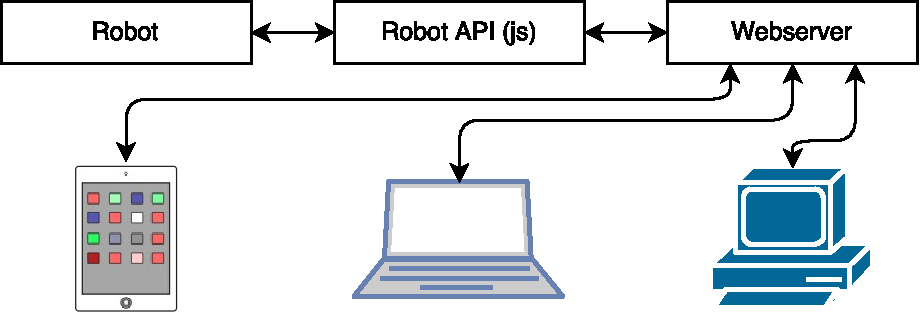
\includegraphics[width = \linewidth]{webgui_architecture}
        \caption{Overview webGUI architecture. The robot's functionalities are exposed with use of the Robot API that is implemented in javascript. The Webserver that is hosting the GUI connects this Robot API to a graphical user interface that is offered to multiple clients on different platforms.}
        \label{fig:webgui_architecture}
\end{figure}

\subsection*{Illustration}



 
\section{Natural Language Interpretation}\label{sec:nli} 
Being able to communicate what you want the robot to do is as vital as having it carry out those tasks successfully, and the more natural this communication is, the easier it is to express the actions. For example, typing:

\begin{lstlisting}
    robot.grasp("drink-123")
\end{lstlisting}

is more cumbersome than saying or typing:

\begin{lstlisting}
    robot grab the drink
\end{lstlisting}

In the first command, you have to know the exact names of the actions the robot can perform. Furthermore, the exact world model identifier of the drink has to be known. If natural language is used, intuition can be used to express the command, without needing further knowledge of the robots internals.

In the Robocup@Home setting, a natural language interpreter is useful for two reasons:

\begin{itemize}
    \item It is vital for using speech recognition (e.g., for the GPSR challenge)
    \item Testing basic actions becomes much easier and less cumbersome. The following command allows us to test object segmentation, classification and manipulation: \texttt{"inspect the cabinet and grab the drink"}
\end{itemize}


A natural language interpreter needs to do two things: parse the structure of the sentence (checking syntax), and converting it to a concise representation of its meaning (semantics). This is done using a feature context free grammar (FCFG). Such a grammar represents the possible structure of the command and at the same time explains how the components of this structure add up into a meaning. An example of such an FCFG is the following:

\begin{lstlisting}
    COMMAND[{"action": A, "entity": X}] -> V[A] NP[X]

    V["inspect"] -> inspect | look at
    V["grab"] -> pick up | grab       
    V["navigate-to"] -> go to | navigate to

    NP[X] -> DET N[X]

    NP[{"id", "cabinet-123"}] -> cabinet-123
    N[{"type": "cabinet"}] -> cabinet
    N[{"type": "drink"}] -> drink

    DET -> the | a
\end{lstlisting}

The capitalized terms represent the structure types encountered within a sentence. For example \texttt{'NP'} stands for 'Noun Phrase', \texttt{'DET'} for 'Determinant', \texttt{'V'} for verb. The rule

\begin{lstlisting}
   A -> B C
\end{lstlisting}   

means that \texttt{A} can be composed of \texttt{B} and \texttt{C}. A vertical bar '|' means one of the terms can be used. For example, \texttt{DET} can be either 'the' or 'a'. The semantics of the grammar are captured within the square brackets. If a rule applies, the variables on the left hand side are replaced with the content of the variables on the right hand side. For example the sentence:

\begin{lstlisting}
   pick up a drink
\end{lstlisting}

will result in the JSON string:

\begin{lstlisting}
    {"action" : grab, "entity" : {"type": "drink"}}
\end{lstlisting}

which expresses that an entity of type drink must be picked up. This command can then be send to the action server, which is responsible for executing actions based on structured JSON commands. Notice that the grammar allows for specifying expressive, generic syntax and semantics. It is for example very easy to provide synonyms for verbs.

Aside from it being easy to use, an explicit data model (grammar) for the interpretation of sentences gives us the added advantage that it can also be used for speech recognition. Limiting the amount of options speech recognition can process greatly benefits the recognition quality. By `telling' speech recognition what it should be able to hear, hearing bad sentences or meaningless commands can be avoided. For example, the grammar above can easily be updated such that "grab the cabinet" cannot be parsed, but "inspect the cabinet" is still possible. By providing speech recognition this updated grammar "grab the cabinet" will never accidentally be heard.

Since new objects may be discovered over the course of a challenge, the grammar is dynamically updated at run-time based on input from the world model. This means that if a table is added to the world model, the id and type of this object are also added as rules to the grammar. For example, in such a case the following rules could be added:

\begin{lstlisting}
    NP[{"id", "table-7"}] -> table-7
    N[{"type": "table"}] -> table
\end{lstlisting}    
    
Allowing interpretation of commands such as:

\begin{lstlisting}
    inspect table-7
    go to the table
\end{lstlisting}

A natural language console was created which allows typing natural commands to the robot. Using the grammar, tab-completion could easily be integrated into this console.

%\section{World Modeling}\label{oo:sec:ed}
%The TUe \acrfull{ed} is a \acrfull{ros} based 3D geometric, object-based world representation system for robots. In itself ED is database system that structures multi-modal sensor information and represents this in an object-based world representation that can be utilized for robot localisation, navigation, manipulation and interaction functions. See Figure \ref{fig:ed} for a schematic overview of \href{https://github.com/tue-robotics/ed}{ED}. %\footnote{\acrshort{ed} is an evolution of \acrfull{wire}, that was created in the FP7 RoboEarth Project. Secondly, ED is utilized within the RoboCup @home competition (also read the \href{https://github.com/tue-robotics/team_description_paper/blob/master/Tech_United_At_Home_TDP_2015.pdf}{TU/e 2015 TDP} for RoboCup). More information, software, installation manual and tutorial can be found on \url{https://github.com/tue-robotics/ed}}
%An elaborate explanation, including tutorials are available at our GitHub website \footnote{\url{http://github.com/tue-robotics}}.
Tech United uses ED in its AMIGO and SERGIO robots that participate (and collaborate) in the @Home league. In previous years, developments have been focussed towards making ED platform independent. As a results ED had been used on the PR2 system, Turtlebot and Dr. Robot systems (X80).
\begin{figure}[h]
    %\vspace{-0.3cm}
	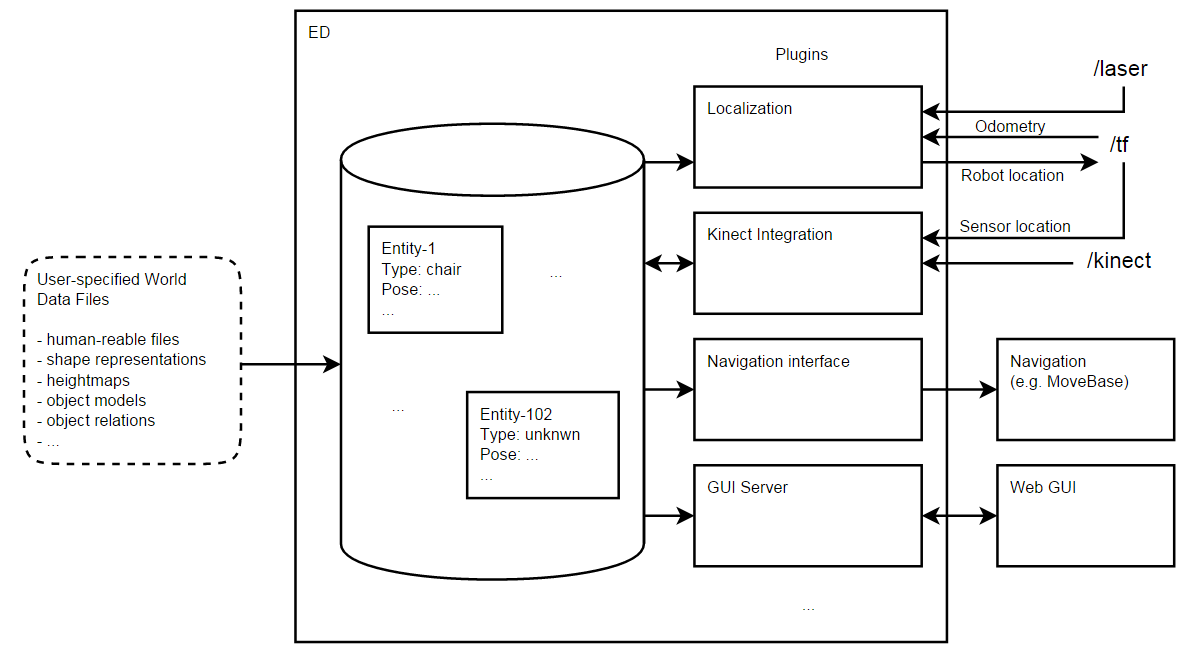
\includegraphics[width = \linewidth]{Figures/ed_overview}
    %\vspace{-1em}
	\caption{schematic overview of TUe Environment Descriptor.}
	\label{fig:ed}
    %\vspace{-0.5cm}
\end{figure}
ED is one re-usable environment description that can be used for a multitude of needed functionalities. Instead of having different environment representations for localization \acrfull{amcl}, navigation (MoveBase), manipulation (MoveIt!), interaction, etc.. An improvement in this single, central world model will reflect in the performances of the separate robot capabilities. It omits updating and synchronization of multiple world models. At the moment different ED modules exist which enable robots to localize themselves, update positions of known objects based on recent sensor data, segment and store newly encountered objects and visualize all this through a web-based \acrshort{gui}.
\begin{figure}[h]
\centering
    %\vspace{-0.3cm}
	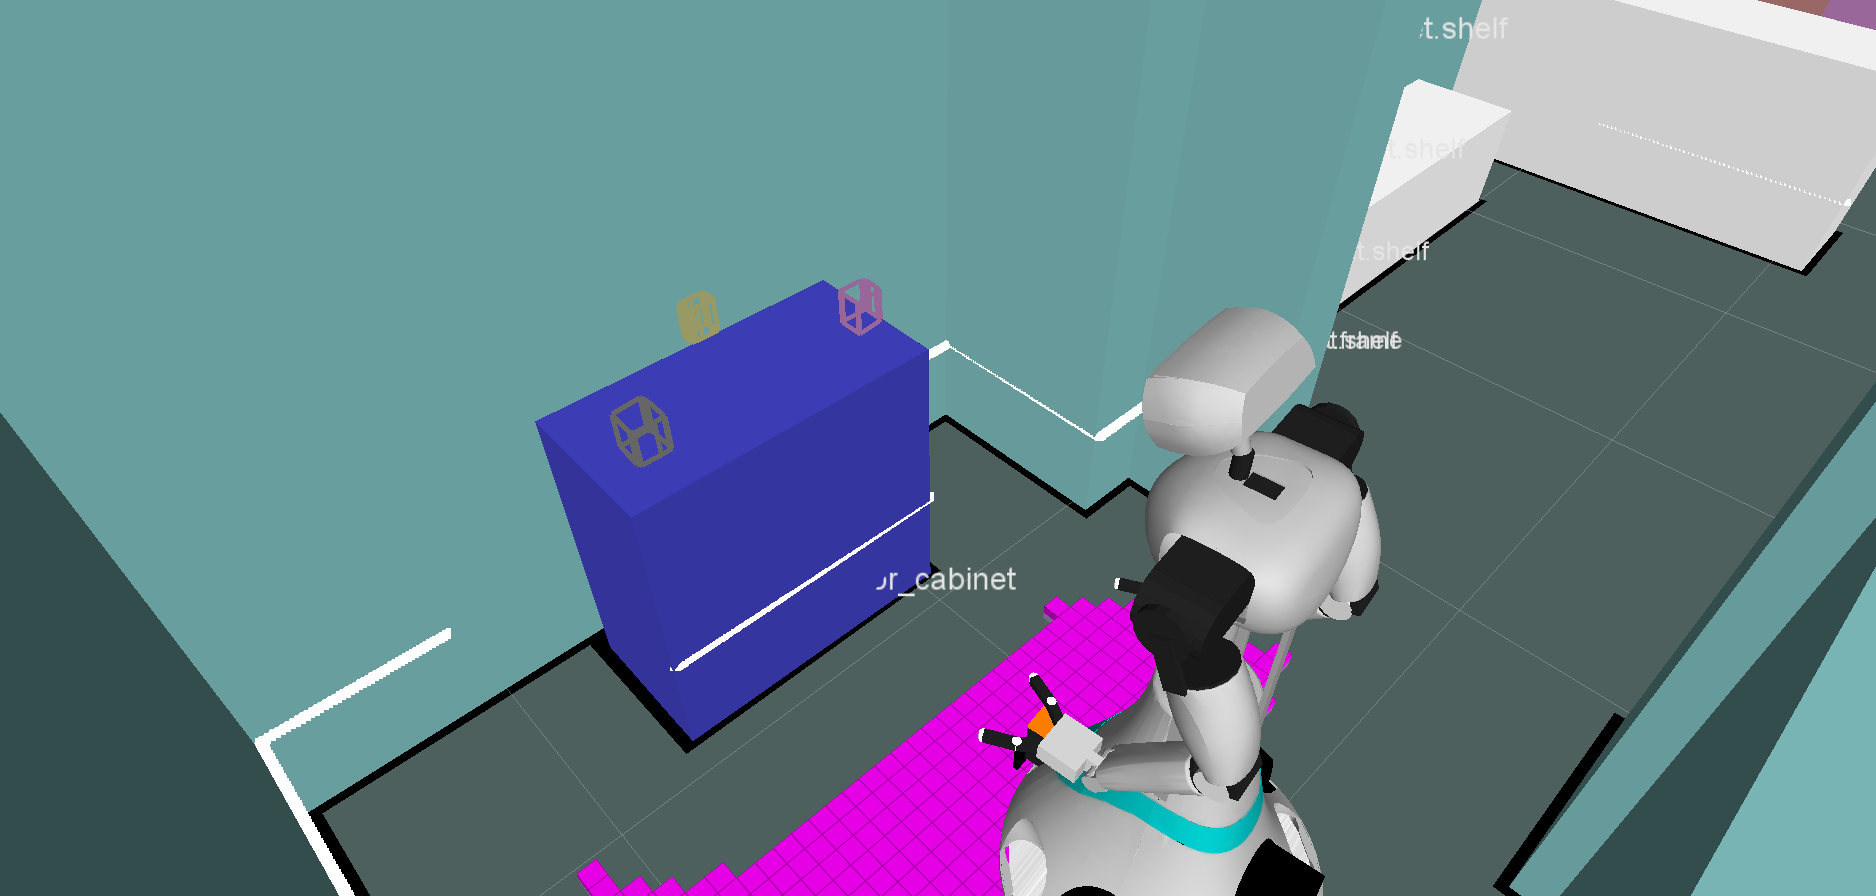
\includegraphics[width = 0.8\linewidth]{Figures/ed_segmentation}
    %\vspace{-0.5em}
	\caption{A view of the world model created with ED. The figure show the occupation grid as well as (unknown) objects recognized on top of the cabinet.}
	\label{fig:ed_segmentation}
    %\vspace{-0.5cm}
\end{figure}


%
%\section{Perception}\label{sec:perception}
%\input{perception.tex}
%
%\section{Navigation}\label{sec:navigation}
%\input{navigation.tex}

\section{Conclusions}
In this paper, this year's main developments of Tech United Eindhoven have been discussed: 
\begin{itemize}
	\item Localization, navigation and object segmentation all benefit from the updating the pose of furniture objects by means of a novel fitting algorithm.
	\item Interaction with the robots is possible from a large variety of platforms due to the WebGUI.
	\item A Natural Language Interpreter allows an easier specification of commands to the robot and a robust speech recognition by excluding meaningless commands from the options that the robot is able to understand.
%	\item A new world model has been developed: Environment Descriptor. By combining semantic and volumetric information about the environment, this world model can be used not only for task planning and execution but also for motion planning.
%	\item Perception algorithms are implemented as `workers' on world model entities which allows for real-time classification of objects.
%	\item One of the benefits of using a volumetric world model is that predefined waypoints have become obsolete. Instead, a goal area can be defined depending on the task and the object at hand, which greatly robustifies navigation.
\end{itemize}
With these improvements, we hope to improve on last year's performance. We are looking forward to RoboCup~2015 in Huefei! 

\section*{Robot Hardware Descriptions}
\begin{figure}[ht]
    \begin{minipage}[t]{0.48\textwidth}
        \centering
%        \includegraphics[height = 6cm, bb = 0 0 590 812]{Figures/AMIGO_BvOF_Cropped.jpg}
        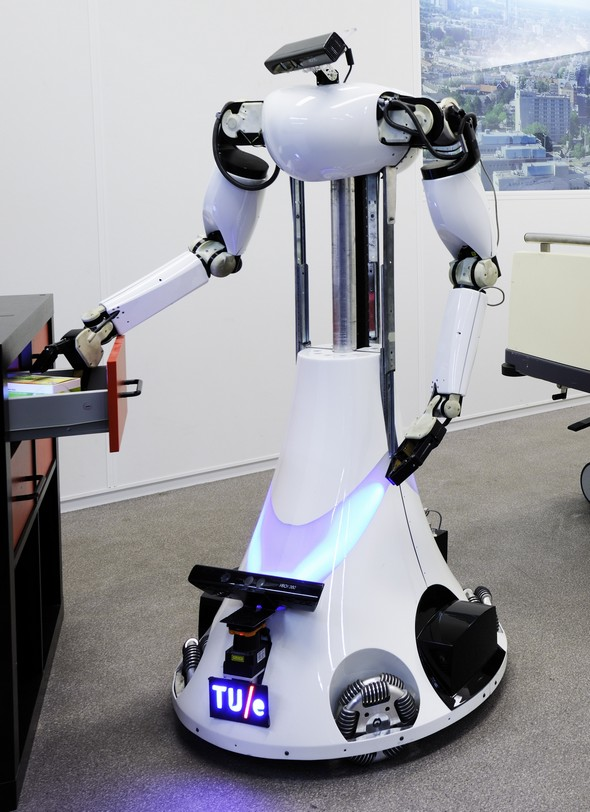
\includegraphics[height = 5.0cm]{Figures/amigo.jpg}
        \caption{The AMIGO robot.}
        \label{fig:amigo}
    \end{minipage}
    \hfill
    \begin{minipage}[t]{0.48\textwidth}
        \centering
%        \includegraphics[height = 6cm, bb = 0 0 687 1069]{Figures/Total_assy_v1.png}
        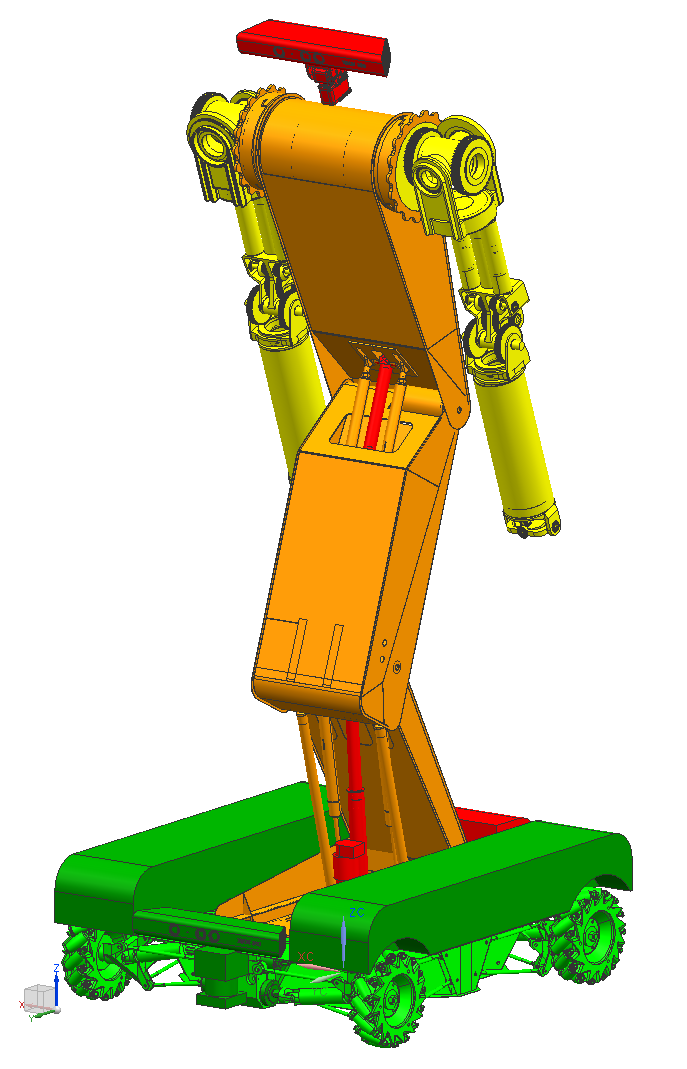
\includegraphics[height = 5.0cm]{Figures/sergio.png}
        \caption{CAD drawing of SERGIO.}
        \label{fig:sergio}
    \end{minipage}
\end{figure}
AMIGO (Autonomous Mate for Intelligent Operations, see Fig.~\ref{fig:amigo}) has competed in RoboCup@Home since 2011. Its design is based on a Middle Size League soccer robot, equipped with two Philips Experimental Robotic Arms mounted on an extensible upper body. Based on our experiences with AMIGO, SERGIO (Second Edition Robot for Generic Indoor Operations, see Fig.~\ref{fig:sergio}) has been developed. The main differences with AMIGO are the use of Mecanum wheels which are compliantly suspended, the torso with two degrees of freedom and the modular setup. The core specifications of AMIGO and SERGIO can be found in Table~\ref{tab:hardwarespec}. More details about the robots can be found on the Robotic Open Platform\footnote{\texttt{http://www.roboticopenplatform.org/}}, where all CAD drawings, electrical schemes and CAD files are published. 

\begin{table}[H]
    \begin{center}
    \caption{Core specifications of AMIGO and SERGIO}
    \label{tab:hardwarespec}
    \renewcommand{\arraystretch}{1.0}
    \setlength{\tabcolsep}{5pt}
        \begin{tabular}{p{0.2\textwidth} p{0.4\textwidth} p{0.4\textwidth}}
            \toprule
            & AMIGO & SERGIO\\
            \midrule
            Name & Autonomous Mate for IntelliGent Operations & Second Edition Robot for Generic Indoor Operations \\
            Base & Fully holonomic omni-wheel platform based on a soccer robot & Fully holonomic Mecanum wheel platform with independent wheel suspension system\\
            Torso & 1 vertical DoF using a ball screw & 1 nearly vertical DoF using a coupled ankle and knee joint, 1 rotational hip joint\\
            Manipulators & 2 7-DoF Philips Experimental Robotic Arms & 2 7-DoF custom arms \\
            Neck & Pan-tilt unit using two Dynamixel RX-28 servo actuators & Pan-tilt unit using two Dynamixel RX-64 servo actuators \\
            Head & Kinect for XBox 360 & Kinect for XBox 360 \\
            External devices & Wireless emergency button & Wireless emergency button \\
            Dimensions & Diameter: $0.75\ \mathrm{m}$, height: $\pm1.5\ \mathrm{m}$ & Base: $0.7\ \mathrm{m}\times0.6\ \mathrm{m}$, height: $\pm1.65\ \mathrm{m}$\\
            Weight & $\pm70\ \mathrm{kg}$ & $\pm70\ \mathrm{kg}$ \\
            Additional sensors & Hokuyo UTM-30LX laser range finder on base and torso & Hokuyo UTM-30LX laser range finder on base and torso (tilting) \\
            Microphone & R{\O}DE Videomic & R{\O}DE Videomic Pro\\
            Batteries & $4\times$ Makita $24\ \mathrm{V},\ 3.3\ \mathrm{Ah}$ & $4\times$ Makita $24\ \mathrm{V},\ 3.3\ \mathrm{Ah}$\\
            Computers & $4\times$ AOpen Mini PC with Core-i7 processor and $8\ \mathrm{Gb}$ RAM & $3\times$ Gigabyte mini ITX board with Core-i7 processor and 	$16\ \mathrm{Gb}$ RAM \\
            \bottomrule
        \end{tabular}
    \end{center}
\end{table}

\section*{Robot Software Description}
An overview of the software used by the Tech United Eindhoven @Home robots can be found in Table~\ref{tab:softwarespec}.
All our software is developed open-source at GitHub\footnote{\texttt{https://github.com/tue-robotics}}

\begin{table}[H]
    \begin{center}
    \caption{Software overview of the robots.}
    \label{tab:softwarespec}
    \vspace{-0.1cm}
    \renewcommand{\arraystretch}{1.0}
    \setlength{\tabcolsep}{5pt}
        \begin{tabular}{p{0.3\textwidth} p{0.7\textwidth}}
        	\toprule
            Operating system & Ubuntu 14.04 LTS Server\\

            Middleware & ROS Indigo~\cite{Quigley2009}\\

            Low-level software & Orocos Real-Time Toolkit~\cite{Bruyninckx2001}\\

            World model & \acrfull{ed}, custom \newline \url{https://github.com/tue-robotics/ed}\\

            Localization & Monte Carlo~\cite{Fox2003} using \gls{ed}, custom \newline \url{https://github.com/tue-robotics/ed_localization}\\

            SLAM & Gmapping: \texttt{http://wiki.ros.org/gmapping}\\

            Navigation & Global: custom A* planner\newline Local: modified ROS DWA~\cite{Fox1997}\\

            Arm navigation & Custom implementation using MoveIt and Orocos KDL\\

            Object recognition & Tensorflow ROS \newline \url{https://github.com/tue-robotics/image_recognition/tree/master/tensorflow_ros} \\

            People detection & Custom implementation using contour matching \\
            Face detection \& recognition & Openface ROS \newline \url{https://github.com/tue-robotics/image_recognition/tree/master/openface_ros} \\
            Speech recognition & Dragonfly + Windows Speech Recognition \newline \texttt{http://code.google.com/p/dragonfly/}\\
            Speech synthesis & Philips Text-to-Speech\\
            Task executors & SMACH\newline\texttt{http://wiki.ros.org/smach}\\
            \bottomrule
        \end{tabular}
    \end{center}
\end{table}


%\section{Introduction}
%While writing the TDP, please focus on your current research and state clear its scientific contribution value and why it is important for you and the league. The length of the TDP is limited to 8 pages. Please leave the hardware and software description for the end of the paper.
%
%Remember that the TDP must contain the following information:
%
%\begin{itemize}
%	\item Description of the hardware and software including a list of integrated externally available components (including commercial products, freeware, Open Source, etc.)
%	\item Innovative technology and scientific contribution
%	\item Photo(s) of the robot
%	\item Focus of research/research interests
%	\item Re-usability of the system for other research groups
%	\item Applicability of the robot in the real world
%\end{itemize}
%
%\section{Background}
%% We are Buy n Large. We have no competitors so no background is required.
%\lipsum[1-3]
%
%\section{BnL Trash Seeker Algorithm (Main research)}
%\lipsum[4-14]
%
%\section{Experiments and results}
%\lipsum[15-20]
%
%\section{Conclusions and future work}
%\lipsum[21-24]
%
%\section*{Robot WALL-E Hardware Description}
%\textit{(In this section briefly describe the software and hardware of the robot)}
%
%Robot WALL-E has the patented \textit{BnL Optimized Design} for garbage recollection. Specifications are as follows:
%
%%\begin{figure}
%%% \begin{wrapfigure}[13]{r}{0.4\textwidth}
%%	\centering
%%	\includegraphics[width=0.4\textwidth]{images/wall-e.jpg}
%%	\caption{Robot WALL-E}
%%	\label{fig:virbot}
%%% \end{wrapfigure}
%%\end{figure}
%
%
%\begin{itemize}
%	\item Base: BnL all-terrain base (differential pair), 2.5m/s max speed.
%	\item Torso: BnL compressor with solar charger.
%	\item Left and right arms: Mounted on torso. 7 DOF, anthropomorphic, BnL Design. Maximum load: 20kg.
%	\item Neck: BnL telescopic neck with pan and tilt.
%	\item Head: 1DOF BnL Expressive Eyes
%	\item External devices: None
%	\item Robot dimensions: height: 1.2m (max), width: 0.7m depth 0.8m
%	\item Robot weight: 50kg.
%\end{itemize}
%
%\textit{Also our robot incorporates the following devices:}
%
%%\begin{itemize}
%%	\item \BnL Battery charge indicator
%%	\item \BnL Auto-focus all-purpose cameras
%%	\item \BnL 7DOF heavy duty fingers
%%	\item \BnL Cockroach
%%\end{itemize}
%
%\section*{Robot's Software Description}
%Please describe in this section the software you are using to control your robot.
%Consider the following example:
%
%\textit{For our robot we are using the following software:}
%
%\begin{itemize}
%	\item Platform: BnL Operating System
%	\item Navigation, localization and mapping: BnL Navigator
%	\item Face recognition: None. Not designed for human interaction.
%	\item Speech recognition: BnL All-purpose recognizer. Please refer to [1, 2, 3]
%	\item Speech generation: None. Not designed for human interaction.
%	\item Object recognition: BnL Trash Seeker Algorithm. See description on previous sections.
%	\item Arms control and two-hand coordination: BnL automatic controller. Please refer to [4, 5, 6]
%\end{itemize}

%\section*{Bibliography}
\bibliographystyle{unsrt}
\bibliography{refs}
\end{document} 